\documentclass[a4paper, 12pt]{report}
\usepackage{graphicx}
\usepackage[utf8]{inputenc}
\usepackage[french]{babel}
\usepackage{mathptmx} %times aves le mode math
\usepackage[T1]{fontenc}
\usepackage{fancyhdr}
\usepackage{amsmath,amsfonts,amssymb, empheq}
\usepackage{eurosym}
\usepackage{booktabs}
\usepackage{wrapfig}
\pagestyle{fancy}
\fancyhead[R]{Université Paris-Est Créteil}
\fancyhead[L]{Projet d'analyse financière}
\usepackage{array,multirow,makecell}
\usepackage{hyperref}
\usepackage{float}  % Nécessaire pour utiliser [H]
\setcellgapes{1pt}
\makegapedcells
\newcolumntype{R}[1]{>{\raggedleft\arraybackslash }b{#1}}
\newcolumntype{L}[1]{>{\raggedright\arraybackslash }b{#1}}
\newcolumntype{C}[1]{>{\centering\arraybackslash }b{#1}} 
%\renewcommand{\thechapter}{\Roman{chapter}}
%\setcounter{chapter}{1} % pour numéroter le chapitre 
\begin{document}

\begin{titlepage}
	\centering
	\begin{center}
		\includegraphics[scale=0.3]{../../../../Pictures/FAC_SEG_rvb}
	\end{center}
	\vspace*{2cm}
	
	\Huge
	
	\textbf{Projet d'analyse financière}
	\vspace{1.5cm}
	
	\Large
Analyse d'Altarea
	
	\vspace{2cm}
	
	\textbf{Nour REBHI, Issa KACHAOU, Enzo CHALAL, Marius AUBERT} \\

	
	
	\vfill
	
	\Large
	
	\textsc{\textbf{Université Paris Est-Créteil}}	 \\
	\textbf{Département d'\'Economie} \\
	\textbf{2025}
	
\end{titlepage}
\thispagestyle{empty}
\newpage
\clearpage
\mbox{}
\thispagestyle{empty}

\tableofcontents

\thispagestyle{empty}
\newpage
\mbox{}
\thispagestyle{empty} %Dernière page vide
%\backmatter
\chapter*{Introduction}
\noindent
Dans le cadre de notre analyse financière, nous nous intéressons à l'indice CAC Small, qui regroupe des sociétés de petite et moyenne capitalisation par rapport aux entreprises des indices CAC 40, CAC Next 20 et CAC Mid 60. Ces entreprises, bien que de taille moyenne, ont une dimension nationale ou internationale, mais restent de taille plus modeste.

Nous nous concentrons particulièrement sur l'entreprise Altarea, fondée en 1994 par Alain Taravella. Altarea est une Société en Commandite par Actions dont les actions sont admises aux négociations sur le marché réglementé Euronext Paris, compartiment A. Le siège social est situé 87, rue de Richelieu à Paris (France). A la fois développeur et investisseur, le Groupe est présent sur les trois principaux marchés de l'immobilier (Commerce, Logement et Immobilier d'entreprise) lui permettant d'être leader des grands projets mixtes de renouvellement urbain en France. Le groupe Altarea opère principalement en France, en Italie et en Espagne.

L'objectif de ce projet est de réaliser une analyse financière comparative entre l'entreprise Altarea et l'indice CAC Small, à partir des données disponibles en 2023.
\thispagestyle{empty}
\newpage
\mbox{}
\thispagestyle{empty} %Dernière page vide
%\backmatter
\chapter{Information de marché}

\section{Analyse graphique des cours}

\subsection{Cours de l'indice CAC Small \& d'Altarea}
\noindent
Durant la première période, l'indice CAC Small fluctue entre 12 000 et 12 400. À partir de la fin août 2023, une tendance baissière s'amorce, culminant en octobre 2023 avec un important pic négatif, où l'indice atteint un creux de 9 800, sa valeur la plus faible pendant toute la période étudiée. Cet écart marque un événement notable.
\begin{wrapfigure}{r}{0.75\textwidth}
	\centering
	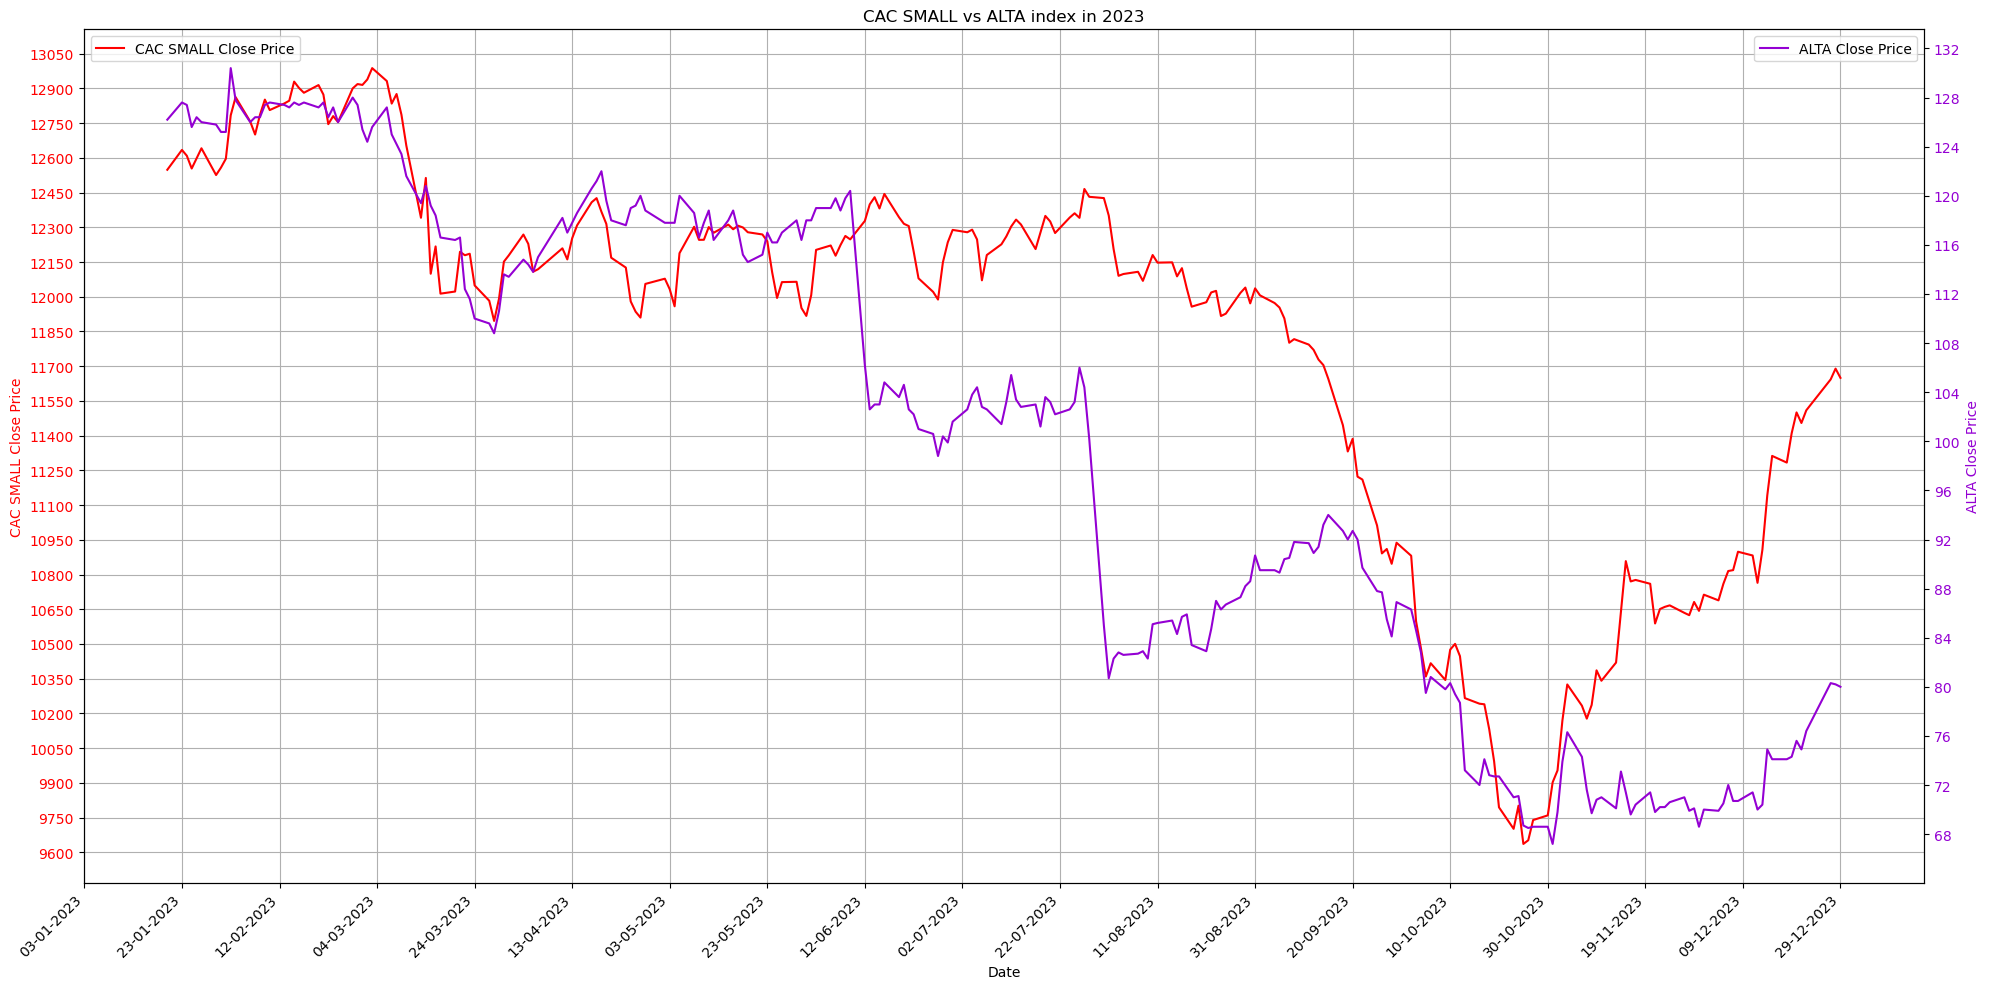
\includegraphics[scale=0.2]{cac_small_return_alta}
	\caption{Tendance générale de l'indice CAC Small et d'Altarea}
\end{wrapfigure}
Ensuite, à partir de novembre 2023, l'indice commence à se redresser progressivement. Ce retour à la normale est suivi d'un pic positif en mai 2024, où l'indice atteint 13 000. Cependant, au début de juin 2024, une chute soudaine survient, faisant descendre le cours à 11 400. Après cette baisse, l'indice évolue dans une fourchette comprise entre 11 700 et 10 200. Toutefois, une tendance à la baisse très marquée devient évidente à la fin de la période étudiée, signalant une nouvelle instabilité dans le cours.
\noindent
Contrairement à l'indice CAC Small, le graphique du cours de l'entreprise Altarea présente des fluctuations plus marquées, illustrant l'instabilité des prix de l'indice. 
\noindent
La première chute soudaine se produit entre fin juillet et début août 2023, où le cours passe de 105 à 86.
\noindent
Ensuite, deux pics à la baisse sont observés, en octobre 2023 et en avril 2024, avec la valeur la plus faible atteignant 68 points. Cependant, à partir d'avril 2024, une tendance haussière se dessine, menant à un pic de 108 points à la mi-mai 2024.

\section{Progression des cours de l'indice et de l'action de l'entreprise en 2023}

\begin{table}[H]
	\centering
	\begin{tabular}{@{}ccc@{}}
		\toprule
		\multicolumn{1}{c}{} & CAC SMALL & ALTAREA \\ \midrule
		Rendement annuel     & -7.161926103961935 \%             & -36.60855784469097 \%           \\ \bottomrule
	\end{tabular}
	\caption{Rendement annuel en 2023}
	\label{tab:my-table}
\end{table}
\subsection{Interprétation des résultats}
\noindent
Le rendement annuel nous permet de quantifier la performance d'un actif sur une période donnée.Une comparaison entre le rendement de l'indice CAC Small et celui de l'action d'Altarea permet de voir comment l'entreprise a performé par rapport à l'ensemble du marché des petites et moyennes entreprises en France.
\noindent
En analysant les données fournies, on constate que le rendement de l'indice CAC Small est de -7 \%, tandis que celui d'Altarea est de -36,6 \%. Cela signifie que, bien que l'indice CAC Small ait enregistré une légère baisse, l'action d'Altarea a sous-performé de manière significative, avec une chute bien plus marquée de son prix. 

Cette différence suggère que, pendant l'année 2023, l'action Altarea a connu des difficultés plus importantes par rapport à l'ensemble des entreprises de l'indice CAC Small, ce qui pourrait indiquer des problèmes spécifiques à l'entreprise ou une volatilité accrue de son action.

\section{Les rendements logarithmiques journaliers}
	
\begin{table}[H]
	\centering
	\begin{tabular}{@{}lrr@{}}
		\toprule
		Date       & Close    & CAC\_SMALL\_return \\ \midrule
		2023-01-20 & 12548.44 & NaN                \\
		2023-01-23 & 12634.24 & 0.681423           \\
		2023-01-24 & 12609.04 & -0.199657          \\
		2023-01-25 & 12553.88 & -0.438424          \\
		2023-01-26 & 12597.22 & 0.344637           \\
		2023-01-27 & 12641.26 & 0.348991           \\
		2023-01-30 & 12525.72 & -0.918194          \\
		2023-01-31 & 12557.78 & 0.255626           \\
		2023-02-01 & 12595.94 & 0.303415           \\
		2023-02-02 & 12783.75 & 1.480029           \\ \bottomrule
	\end{tabular}
	\caption{Les rendements logarithmiques journalier du CAC SMALL}
	\label{tab:my-table1}
\end{table}

\begin{table}[H]
	\centering
	\begin{tabular}{@{}lrr@{}}
		\toprule
		Date         & \multicolumn{1}{l}{Close} & \multicolumn{1}{l}{ALTA\_return} \\ \midrule
		2023-01-20   & 126.2                     & NaN                              \\
		2023-01-23   & 127.6                     & 1.103242                         \\
		2023-01-24   & 127.4                     & -0.156863                        \\
		2023-01-25   & 125.6                     & -1.422949                        \\
		2023-01-26   & 126.4                     & 0.634923                         \\
		2023-01-27   & 126.0                     & -0.316957                        \\
		2023-01-30   & 125.8                     & -0.158856                        \\
		2023-01-31   & 125.2                     & -0.478089                        \\
		2023-02-01   & 125.2                     & 0.000000                         \\
		2023-02-02 & 130.4                     & 4.069419                         \\ \bottomrule
	\end{tabular}
	\caption{Les rendements logarithmiques journaliers d'Altarea}
	\label{tab:my-table2}
\end{table}

\section{Statistiques descriptives}
\noindent
L'analyse descriptive des données, comme les rendements de l'indice CAC Small et de l'action Altarea, permet d'obtenir un aperçu de la performance passée de ces actifs, notamment à travers des statistiques telles que la moyenne, la variance ou l'écart-type. Ces statistiques révèlent non seulement les tendances de rendement, mais aussi la volatilité associée à chaque actif.

En finance, cette analyse est essentielle pour comprendre le couple rendement-risque, qui est essentiel pour évaluer l'attractivité d'un investissement. Les investisseurs cherchent donc à trouver un équilibre entre un rendement attractif et un niveau de risque acceptable, ce qui constitue l'un des principes fondamentaux de la gestion de portefeuille en finance.

\begin{table}[H]
	\centering
	\begin{tabular}{@{}ccc@{}}
		\toprule
		& \multicolumn{1}{c}{CAC\_SMALL\_return} & \multicolumn{1}{c}{ALTA\_return} \\ \midrule
		Moyenne                  & -0.030964                              & -0.189934                        \\
		Variance                 & 0.6957478346068363                     & 4.6517446360651125               \\
		Ecart-type               & 0.834115                               & 2.156790                         \\
		Skewness                 & -0.2655809514495039                    & -2.467476709793943               \\
		Kurtosis                 & 1.248182446640819                      & 17.52605583910445                \\
		Coefficient de variation & 11.35755661                            & 26.90645161                      \\ \bottomrule
	\end{tabular}
	\caption{Statistiques descriptives}
	\label{tab:my-table4}
\end{table}

\subsection{Interprétation des statistiques}

\subsubsection{Moyenne}
\noindent
En 2023, les deux indices, le CAC Small et Altarea, affichent un rendement moyen négatif. Cependant, Altarea (-0.189934) présente une performance significativement plus faible que celle de l'indice CAC Small (-0.030964).

\subsubsection{Écart-type}

Pour les rendements logarithmiques journaliers de CAC Small, l'écart-type est de 0.834115, ce qui indique que les rendements peuvent s'écarter de cette valeur par rapport à la moyenne.
Pour Altarea, l'écart-type est de 2.156790, ce qui suggère une plus grande volatilité des rendements, les écartant davantage de la moyenne.

Cependant, on ne peut pas directement comparer ces deux écarts-types, car les moyennes des deux séries sont différentes. Afin de comparer correctement la volatilité relative de ces deux indices, il est nécessaire de calculer le coefficient de variation, qui standardise l'écart-type par rapport à la moyenne.

\subsubsection{Coefficient de variation (\( CV \)) }

\[ CV=\frac{\sqrt{\frac{\sum(x_i-\bar{x})^2}{N}}}{\frac{1}{N}\sum x_i}
 \]
Avec les coefficients de variation on peut comparer pour voir laquelle a la plus grande volatilité relative.

Le CAC Small a une volatilité relative plus élevée qu'Altarea, même si l'écart-type d'Altarea est plus grand en valeur absolue. Cela signifie que le rendement de CAC Small présente plus de fluctuations proportionnelles.

\subsubsection{Skewness}
\noindent
Pour CAC Small, la skewness négative de -0.2655 suggère une légère tendance vers des rendements plus fréquents et négatifs. Cela indique que les rendements tendent à être légèrement plus bas que la moyenne, mais cette asymétrie est relativement modérée.

En revanche, la skewness d'Altarea est bien plus négative (-2.4674), ce qui reflète une asymétrie négative plus marquée. Cela signifie que la distribution des rendements présente une concentration plus importante d'outliers en dessous de la moyenne, et que la distribution est déviée vers des valeurs faibles. En d'autres termes, Altarea a connu une fréquence plus élevée de fortes baisses que de hausses.

\subsubsection{Kurtosis}
\noindent
La kurtosis du CAC Small est relativement faible (1.248), ce qui suggère que la distribution des rendements est proche d'une distribution normale.

Cependant, la kurtosis d'Altarea  est extrêmement élevée (17.526), bien au-dessus du seuil de 6, ce qui indique un problème majeur de valeurs extrêmes (outliers). Cette forte kurtosis suggère que la distribution d'Altarea est caractérisée par des queues épaisses, ce qui signifie que la probabilité d'événements éloignés de la moyenne est élevée. Cela signifie que la série des rendements d'Altarea  a connu de nombreux événements extrêmes au cours de la période étudiée.

\section{Relation entre les rendements}
\noindent
Pour analyser la relation entre les deux séries de rendements, nous avons réalisé un nuage de points. 
\begin{figure}[H]
\begin{center}
	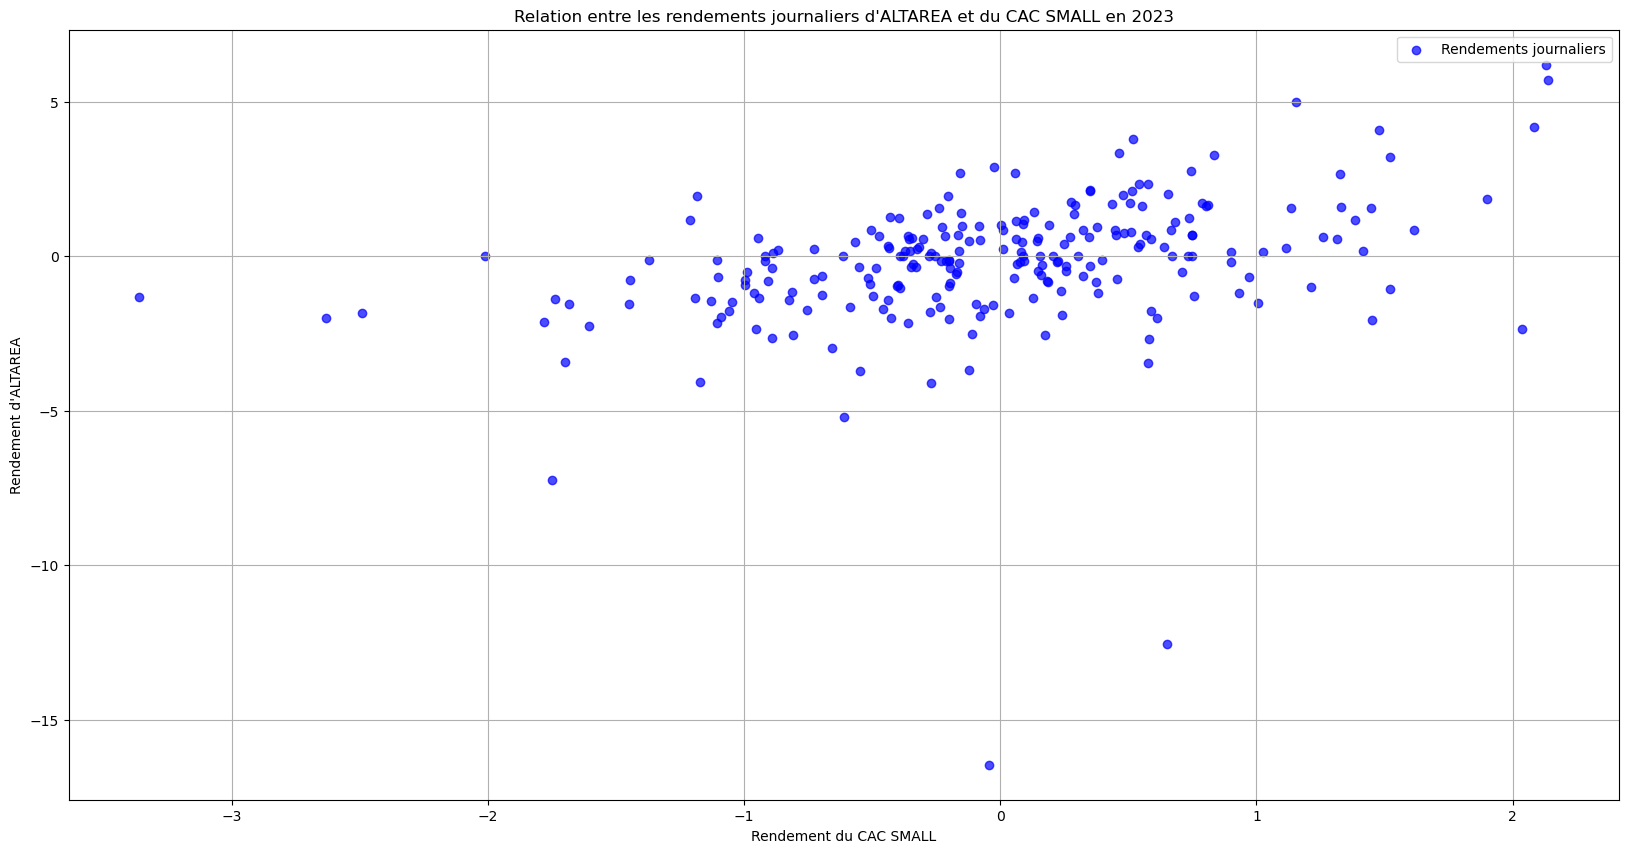
\includegraphics[scale=0.3]{scatter_plot_cacs_alta}
	\caption{Relation entre les rendements d'Altarea et du CAC SMALL}
\end{center}
\end{figure}
Les points du graphique suivent une tendance linéaire, presque alignés autour d'une droite, ce qui indique une relation linéaire entre les rendements de l'action et de l'indice. 
En outre, la droite montre une pente positive, ce qui indique que l'action évolue généralement dans le même sens que l'indice : lorsque l'indice progresse, l'action a tendance à suivre cette tendance haussière, et inversement.

\chapter{Information comptable}
\noindent
Dans le rapport annuel de la société ALTAREA, relatif à l'exercice clos le 31 décembre 2023, il est mentionné que les commissaires aux comptes ont effectué l'audit des comptes annuels de l'entreprise. 
Ces derniers ont certifié que les comptes, au regard des règles et principes comptables français, donnent une image fidèle du résultat des opérations de l'exercice 2023, ainsi que de la situation du patrimoine et de la santé financière de la société à la fin de l'année. 
Les comptes consolidés ont été arrêtés par la Gérance le 27 février 2024, après avoir été examinés par le Comité d'Audit et le Conseil de Surveillance, puis validés lors de l'Assemblée Générale de la société.



























\end{document}